\documentclass[titlepage]{article}
\usepackage{graphicx}
\usepackage{geometry}
\usepackage{cite}
\usepackage{url}
\usepackage{algorithm}
\usepackage{algpseudocode}
\usepackage{wrapfig}
\usepackage{multicol}
\usepackage[colorlinks]{hyperref}
\usepackage{xspace}

\makeatletter
\g@addto@macro{\UrlBreaks}{\UrlOrds}
\makeatother

\newcommand{\ohw}{\textit{one-hit wonder}\xspace}
\newcommand{\nos}{\textit{nostalgia}\xspace}
\newcommand{\sea}{\textit{seasonal}\xspace}
\newcommand{\ris}{\textit{rising}\xspace}
\newcommand{\fad}{\textit{fading}\xspace}
\newcommand{\const}{\textit{constant}\xspace}

\geometry{
 a4paper,
 total={170mm,257mm},
 left=20mm,
 top=20mm,
 }

\title{
Understanding Collective Memory Patterns by Analyzing View Patterns of People’s Pages on the English Wikipedia \\ \vspace{5mm}
\large{Final Project for the Course \textit{The Art of Analyzing Big Data}}}
\author{Netanel Madmoni}
\date{April 2024}

\begin{document}

\maketitle

\section{Introduction}
\subsection{Wikipedia Statistics as Collective Memory Measures}
There are many works on the concept of \textit{collective memory}. Dating back to the 1920s, this concept of memory extends beyond individual recollection to encompass the shared experiences and representations of communities, cultures, and societies \cite{igarashiTwophaseModelCollective2022}. In 2009, Pentzold \cite{pentzoldFixingFloatingGap2009} proposed 'to interpret the web-based encyclopedia Wikipedia as a global memory place', as it lets locally disconnected members to combine their knowledge and perspectives into one collective memory in the cyberspace. Following this notion, many researchers often used Wikipedia statistics as a proxy for the collective memory \cite{yasseriCollectiveMemoryDigital2022} and attention \cite{ruprechterPoorAttentionWealth2023} \cite{gildersleveNewsHistoryIdentifying2023}.

\subsection{Time Series Pattern Extraction \& Approximation}

\begin{wrapfigure}{r}{0.4\textwidth}
    \centering
    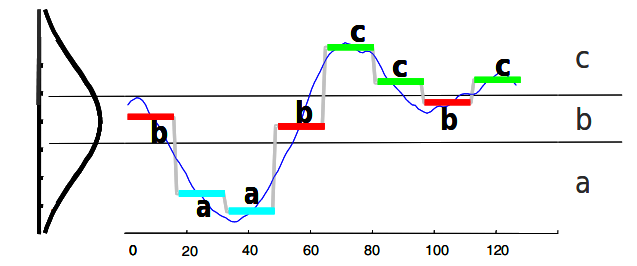
\includegraphics[width=0.8\linewidth]{figures/sax_illustration_lin_etal.png}
    \caption{SAX algorithm illustration. The time series is discretized and mapped to specified breakpoints, resulting in the representation \textbf{baabccbc}. Source: \cite{linExperiencingSAXNovel2007}}
    \label{fig:sax-illustration}
\end{wrapfigure}
Pattern extraction from time series is a important aspect of time series analysis in all areas of time-series- or signal-processing- related research with many real-world applications. Many algorithms have been developed over the years for both local and global pattern extraction for a variety of different tasks, such as classification \cite{geurtsPatternExtractionTime2001} \cite{yeTimeSeriesShapelets2009} and clustering \cite{ulanovaScalableClusteringTime2015}.
One of the useful tools used for time series analysis and pattern extraction is time series approximation. It is used not only for overcoming technical limitations such as computation time and storage space, but can also be used for representing time-series data in a meaningful way for specific tasks such as pattern extraction and features discovery. Symbolic ApproXimation (SAX) is a relatively simple and intuitive method for time series approximation proposed by Lin \textit{et al.} \cite{linExperiencingSAXNovel2007}. The method reduces the dimensionality of a time series by dividing it into equal sized 'frames' and calculating the mean value for each frame, and then discretizing the reduced series into predetermined bins. See Figure \ref{fig:sax-illustration} for an illustration of the algorithm.

\subsection{Contribution}
In this work I identify and investigate the commonness of six intuitive different page views patterns of around two million Wikipedia pages of persons over nine years (2015-2023), using publicly available page views information and pages data. My goal is to reveal properties of the collective memory in regards to people, and have a better intuitive understanding of different groups of pages by characterizing the patterns that are present in their views over time.

\section{Method}
\subsection{Data Description \& Acquisition}
In this project I use three sources of data:
\begin{enumerate}
    \item \textbf{English Wikipedia page view data} - from a public dataset hosted on Google BigQuery\footnote{Google cloud bucket: \texttt{gs://cloud-samples-data/third-party/wikimedia/pageviews}.\label{footnote:bigquery}}. The dataset contains an hourly view count of all of the pages on Wikipedia over the years 2015-2023. The granularity of this dataset is at the hourly level, which is too high for the purpose of this project. I've taken a monthly sum of the views for each entity, resulting in a total of over 200 million data points across over 2 million rows (later filtered to around 1.5 million rows). 
    \item \textbf{Wikidata entity data} - a public dataset containing information about Wikidata entities. Also hosted on Google BigQuery\textsuperscript{\ref{footnote:bigquery}}.
    \item \textbf{Database of notable people} - a cross-verified database published in 2022 by Laouenan \textit{et al}. \cite{laouenan_cross-verified_2022}. The database contains a verified list of people on Wikidata and their properties. Due to the importance and cleanliness of this information, I decided to only use the pages that are present in this database.\footnote{Also due to the Wikidata entity data being messy, incomplete and sometimes false, the verified database is the main source of the information in regards to entity properties.}
\end{enumerate}

The raw data was cleaned and transformed in preparation for the pattern extraction. For a detailed description of the data fields and cleaning process, refer to the accompanying code files, \texttt{notebook 1} in the \nameref{supplementary} section.


\subsection{Pattern Classification}
In this section I describe the patterns I've selected to identify as well as the methods for classifying a pattern.

\subsubsection{The Patterns}
\begin{wrapfigure}{r}{0.4\textwidth}
    \centering
    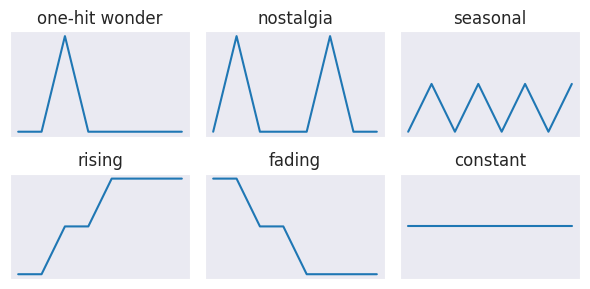
\includegraphics[width=\linewidth]{figures/patterns.png}
    \caption{Illustrations of each of the patterns.}
    \label{fig:patterns-illustration}
\end{wrapfigure}
I decided to focus on the following patterns:


\begin{itemize}
    \item \textit{One-hit wonder pattern} - the term 'one-hit wonder' is taken from the music industry. Originally it refers to a band or an individual that became popular due to a single piece of work going viral. In this work I am borrowing this term to describe a page of a person that received one big 'peak' of views during the lifetime of the page.
    \item \textit{Nostalgia pattern} - similar to \textit{one-hit wonder}, but here the page views had two big "peaks" of views during its lifetime, emulating the "nostalgia" phenomenon.
    \item \textit{Seasonal pattern} - where an entity has at least one strong seasonal components in the views its page receives.
    \item \textit{Rising pattern} - where an entity has an upward trend in its views over time.
    \item \textit{Fading pattern} - where an entity has an downward trend in its views over time.
    \item \textit{Constant / no pattern} - where an entity has no particular pattern in its page views over time (the default).
\end{itemize}
A simple illustration of each pattern is shown in Figure \ref{fig:patterns-illustration}.


\subsubsection{Assumptions}
For simplicity, I decided to assume the following: 1) An entity can have more than one pattern, as long as the patterns don't contradict each other (for example, a person can have both \ohw and \sea, but not \ohw and \nos, or \ris and \fad, as they are contradictory by definition). 2) The patterns are independent of the absolute volume of the series, meaning, popular pages (high sum of views over the years) as well as less popular can have the same pattern. In other words, it is the shape that I am interested in, regardless of its absolute values. 3) Each pattern spans across the entirety of the series, i.e., the subject of classification is the series as a whole, rather than just subsequences of it is (as opposed to, say, shapelets \cite{yeTimeSeriesShapelets2009}). In future work it might be worth questioning all of these assumptions.


\subsubsection{Determining the Pattern of Each Series \label{section:pattern-determination}}
In order to determine the category into which each page views time-series fall, I first calculate the symbolic approximation (SAX) of each time series, classifying each observation into one of two bins: \textit{high} and \textit{low}. I then count the number of observations in the \textit{high} bin. This is what I consider as the number of 'significant' peaks. If there is a singular peak, then the series is classified as \textit{one-hit wonder}. If there are two peaks, then the series is classified as \textit{nostalgia}. It is important to note that I've considered clusters of observations will to count as a singular peak if they are within distance $d$ from each other, for a predetermined $d$ (here I've chosen $d = 3$, meaning that peaks within the same quarter-year will count as a single peak).

Next, i test for the \textit{seasonal} pattern. To determine if a series has a significant seasonal component, I use the autocorrelation function (ACF) for lags $d + 1 = 4$ to 21 and calculate the confidence interval for each autocorrelation one at significance level .95, using the Ljung–Box test \cite{ljungMeasureLackFit1978}. If the confidence interval's lower bound of any autocorrelation is positive, then that series is considered to have a significant seasonal component and is classified as \textit{seasonal}.

Then, I perform a simple linear regression on the series. If the regression's p-value is significant, then that series is classified as \textit{rising} or \textit{fading}, according to the slope of the regression.

Any series that hasn't been classified yet, will be classified as \textit{constant}.

% The procedure of the pattern classification is described in Algorithm \ref{alg:pattern-classification}.
Figure \ref{fig:examples} shows a few (good\footnote{I admit that a lot of examples are not classified in an intuitive manner, see more on section \nameref{section:discussion}.}) examples for various patterns.

% \begin{algorithm}[H]
%     \caption{Pattern Classification}
%     \label{alg:pattern-classification}
%     \begin{algorithmic}
%     \State \textbf{Data:} $\mathbf{x}$ - the time series of page views for an individual's Wikipedia page.
%     \If{number of peaks in sax($\mathbf{x}$) = 1}
%         \State \Return \textit{one-hit-wonder}.
%     \ElsIf{number of peaks in sax($\mathbf{x}$) = 2}
%         \State \Return \textit{nostalgia}.
%     \ElsIf{seasonality}
%         \State \Return \textit{seasonal}.
%     \Else
%     \State calculate linear regression slope $\beta$, p-value $p$.
%         \If{$p >.05$ and $\beta > 0$}
%             \State \Return \textit{rising}.
%         \ElsIf{$p >.05$ and $\beta < 0$}
%             \State \Return \textit{fading}.
%         \Else
%             \State \Return \textit{constant}.
%     \EndIf
%     \EndIf

%     \end{algorithmic}
% \end{algorithm}

\begin{figure}[H]
    \centering
    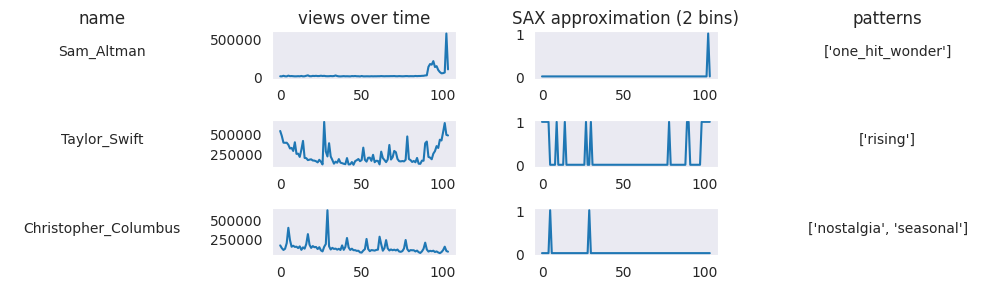
\includegraphics[width=\linewidth]{figures/examples.png}
    \caption{A few examples for various patterns.}
    \label{fig:examples}
\end{figure}

\subsection*{A Note on Optimization}
Since the data is very large in volume, I've employed different techniques for achieving satisfactory results in a reasonable amount of time and memory space. These include working with \texttt{parquet} files and using the \texttt{Polars} package \cite{Pola-Rs} for data transformation, and more importantly: defining relatively simple, easy to calculate measures.

\section{Results}
For the dataset as a whole, the \ohw pattern was the most common one (after the default \const pattern). A close second is the \sea pattern, followed by the \nos, \fad and \ris patterns, in that order. Figure \ref{fig:global-dist} shows the number of occurrences for each of the patterns in the dataset as a whole. I discuss these results in Section \ref{section:discussion}.

\begin{figure}[H]
    \centering
    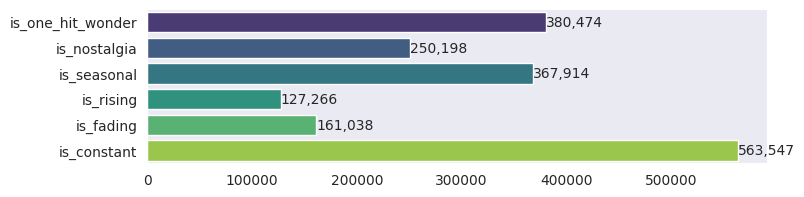
\includegraphics[width=0.7\linewidth]{figures/global_distribution.png}
    \caption{Count of patterns over the entire dataset.}
    \label{fig:global-dist}
\end{figure}

Next are the pattern distributions by some individual properties\footnote{I've chosen some of the interesting properties to display. Distributions of the patterns by other properties can be found in the code in the \nameref{supplementary}, \texttt{notebook 2}.}. Figure \ref{fig:gender} shows the distributions by gender. Note that in all of the following figures, the counts have been normalized for each group (divided by the total number of patterns present in that group).

\begin{figure}[H]
    \centering
    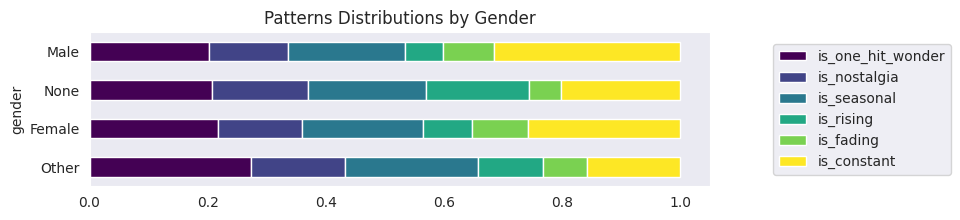
\includegraphics[width=0.6\linewidth]{figures/genders.png}
    \caption{Count of patterns by gender.}
    \label{fig:gender}
\end{figure}

Although they seem very similar, there is a statistically significant difference in proportions between the male and female group, i.e., the proportion of each pattern (except for the default pattern \const) within the male group was significantly smaller than that proportion in the female group ($p \ll\ .0001$).

Below (Figure \ref{fig:occupation} are the normalized pattern counts by occupation.

\begin{figure}[H]
    \centering
    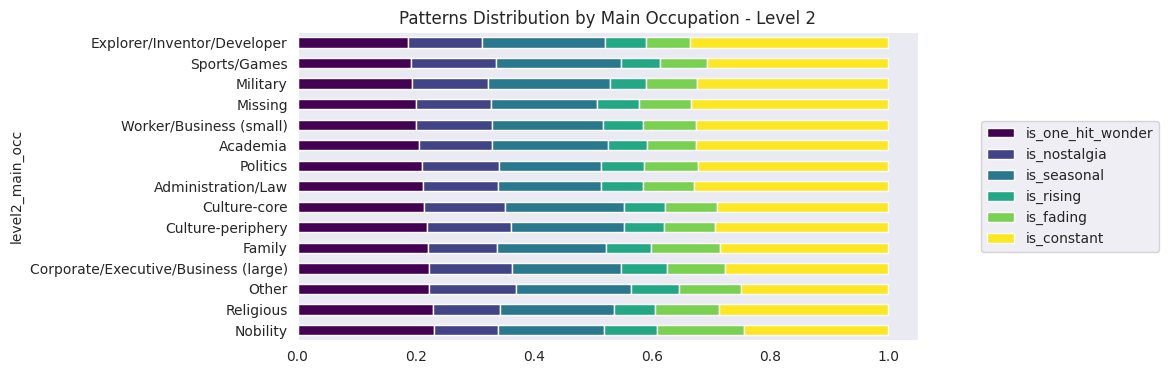
\includegraphics[width=\linewidth]{figures/occupation_2.png}
    \caption{Count of patterns by occupation.}
    \label{fig:occupation}
\end{figure}

It seems that the proportions are similar between groups, however 2/3 of the combinations are significantly different between groups. It is interesting to see that the occupations \textit{nobility} and \textit{religion} have the most \ohw-s, although being two groups with little members.

An interesting observation for both gender and occupation\footnote{As well as other properties present in the supplementary material, \texttt{notebook 2}.}, while statistically different, the proportions within each group seem roughly similar to the global proportions presented in Figure \ref{fig:global-dist}. This is not the case for the distributions by birth period (Figure \ref{fig:birth-period}).

\begin{figure}[H]
    \centering
    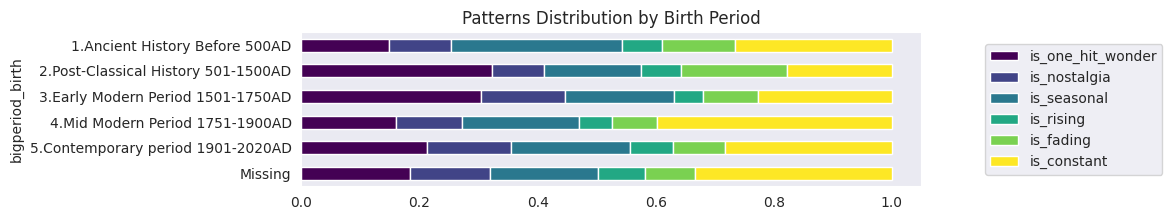
\includegraphics[width=\linewidth]{figures/birth_period.png}
    \caption{Count of patterns by birth period.}
    \label{fig:birth-period}
\end{figure}

As it seems (and perhaps counter-intuitive), in years 501-1750 AD, the proportion\footnote{Remember: these are normalized proportions by group, and not absolute numbers.} of \ohw-s is much larger relative to the other eras. Also worth noting that the seasonal pattern is more prominent for people living before 500AD. I discuss this in Section \ref{section:discussion}.

Finally, we can look at the patterns distributions by Laouenan \textit{et al.}'s \cite{laouenan_cross-verified_2022} \textit{notability rank} of a person. It is a measure comprised of the number of Wikipedia editions of each individual, the length in all available Wikidata biographies for the individual, the average number of biography views for them between 2015 and 2018 in all available language editions, the number of non-missing items retrieved from Wikipedia or Wikidata for birth date, gender and domain of influence. I have grouped the ranks into ten bins. The normalized pattern count for each bin is presented in Figure \ref{fig:notability}.

\begin{figure}[H]
    \centering
    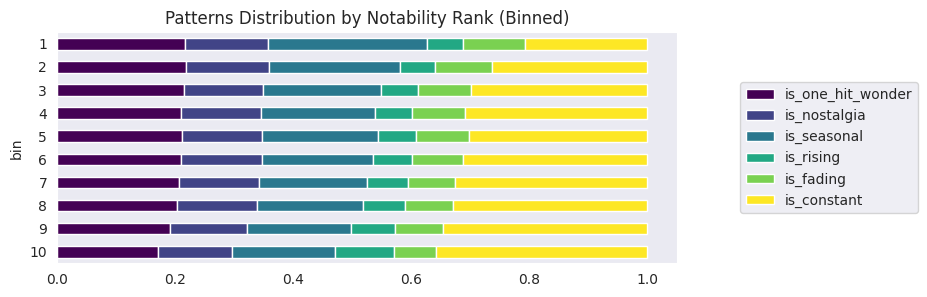
\includegraphics[width=0.8\linewidth]{figures/notability.png}
    \caption{Count of patterns by binned notability rank. Lower bin number means more notable.}
    \label{fig:notability}
\end{figure}

It seems that the percentage of the default non-pattern \const is correlated with notability rank (see Figure \ref{fig:notability-reg}), meaning that less notable people have more constant patterns. By that logic, the more notable a person is, it is more likely to have one of the 'special' patterns.

\begin{figure}[H]
    \centering
    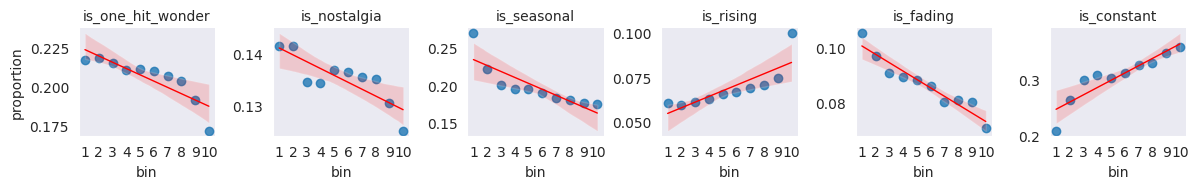
\includegraphics[width=\linewidth]{figures/notability_reg.png}
    \caption{Regression plots describing the proportion of each pattern by binned notability rank. Lower bin number means more notable. Most of the patterns have decreasing proportion with rank, meaning the pattern is more present for more notable people.}
    \label{fig:notability-reg}
\end{figure}

\section{Discussion \& Future Work \label{section:discussion}}
In this work, in order to better understand the collective memory in regards to people, measured by Wikipedia page views, I presented a way to classify people's page views on the English Wikipedia into six simple patterns, using intuitive and statistical measures. I was able to classify a large portion of pages into one of five 'special' patterns: \ohw, \nos, \sea, \ris, and \fad. Surprisingly, out of those five, the largest group in the dataset as a whole was the \ohw group, meaning the page had a high number of views in a single short period during the last nine years. This might reveal an important aspect of our 'collective memory': does the memory shifts globally from one subject to another in a short period of time?

For the seasonal pattern, the presence of seasonality in some people's Wikipedia articles might be due to a academic interest in these people that fluctuated over the academic year \cite{segevSeekingScienceInformation2012}, which is a reasonable speculation for people from earlier historical eras, or real world-events happening seasonally for living people.

This work should be considered a preliminary investigation. There are many interesting ways in which it can be improved. Admittedly, for many samples, the chosen pattern was not very intuitive. I think this is might be due to the fact that page views, especially over nine years, have more complex patterns that can't be defined by a single 'shape' over their entire lifespan (local patterns might be more robust and intuitive than the global patterns).
The selection of the minimum distance between peak clusters described in Section \ref{section:pattern-determination} also seems to have a big impact on the classification. The patterns themselves and the way of extracting them might need to be assessed as well. I have treated the patterns as independent of the absolute number of views in the series, an assumption worth questioning. Finally, it would be interesting to try to develop a machine learning model that can predict a views pattern from a person's properties such as occupation, gender, etc.

I believe this project can provide a solid foundation to a better understanding of the view patterns on Wikipedia and a window to the workings of our global memory.

\section*{Acknowledgements}
I've used the assistance of generative AI (ChatGPT) in the writing of some of the code and this report.

\section*{Supplementary Material} \label{supplementary}
\begin{itemize}
    \item \textbf{Data.} I have uploaded both the page view data and the Wikidata entity data to Kaggle, and they are available in this dataset: \url{https://www.kaggle.com/datasets/netanelmad/wikipedia-people-page-views-data}. The verified people dataset by Laouenan \textit{et al.} \cite{laouenan_cross-verified_2022} is available at \url{https://data.sciencespo.fr/dataset.xhtml?persistentId=doi:10.21410/7E4/RDAG3O}.
    \item \textbf{Code.} My code is available at the GitHub repository: \url{https://github.com/MNetanel/wikipedia-people-page-views-patterns}.
\end{itemize}


\newpage
\bibliographystyle{IEEEtran}
\bibliography{citations}

\end{document}
